	
\section{Discussion}

\subsection{Potential Solutions}

\begin{itemize}
	\item[---] \textbf{Public blockchains} are large distributed networks that are run through a native token such as bitcoin or ether. Anyone can participate and the community maintains its open-source code. The two largest public blockchains are Ethereum and Bitcoin. They are open for anyone to participate at any level and have open-source code that their community maintains.
	% rewrite and add section about composer
	\item[---] \textbf{Permissioned blockchains} define role based access control for individuals in the network and uses native tokens.  HyperLedger Composer, an open-source framework for permissioned blockchains, is used for smart contracts and for blockchain application development \cite{hyperledgerComposer:Online}. One use case is an accounting system that calculates payment, while hiding that information from unrelated organizations.  \hfill \break % Their core code may or may not be open source.
	\begin{figure}[ht]
	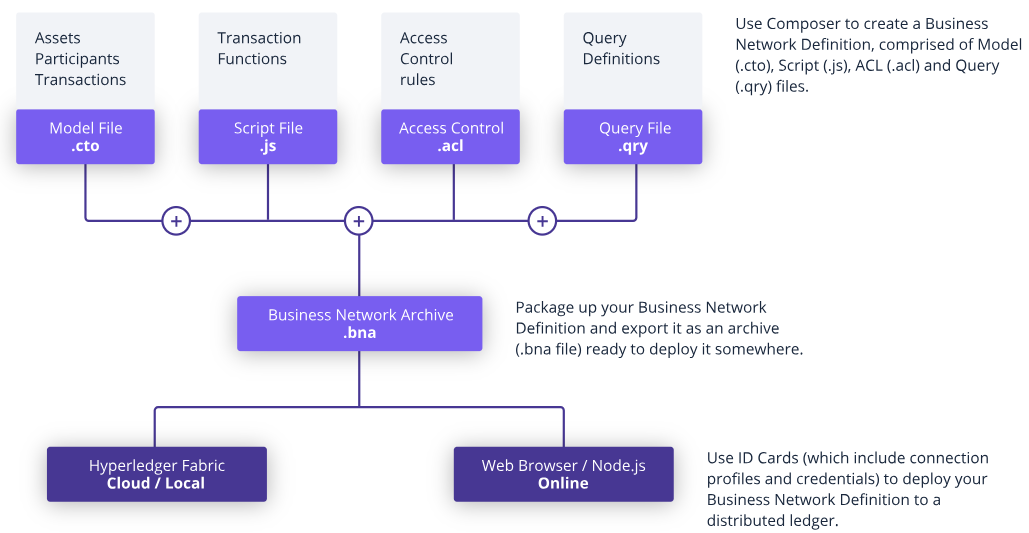
\includegraphics[width=1\linewidth]{Diagrams/composer-arch.png}
	\caption{Architecture of Hyperledger composer}
	\end{figure}
	\item[---] \textbf{Private blockchains}  membership is tightly controlled and lacks a native token. Useful for consortiums with trusted associates and exchanging confidential information, however, less powerful because it is supported by limited private resources. Large organizations such as governments will likely use these extensively.
\end{itemize}

\newpage 
\subsection{Initial Assessment}
% Discuss how it is significantly more accessible for money to issue their own currencies, ICOs

% Explain how much it costs to how a bunch, like 5%, getting an automatic system will be cheaper as wages will not be paid, cover cost of gas
% "Gas" is the name for a special unit used in Ethereum. It measures how much "work" an action or set of actions takes to perform: for example, to calculate one Keccak256 cryptographic hash it will take 30 gas each time a hash is calculated, plus a cost of 6 more gas for every 256 bits of data being hashed. Every operation that can be performed by a transaction or contract on the Ethereum platform costs a certain number of gas, with operations that require more computational resources costing more gas than operations that require few computational resources.

% https://ethereum.stackexchange.com/questions/3/what-is-meant-by-the-term-gas

Determining which platform is best for smart contracts should be done using a weighted decision matrix, based on the particular application. For internal processes such as supply chains, a private blockchain makes sense (data cannot be changed) and cryptographic auditing with known identities (public keys). For a trustless system that verifies every transaction, using a public blockchain is essential. In comparison, role-based access control is feasible by using a permissioned blockchain. \hfill \break
%\hfill \break 

Despite the slow speed of the public blockchain, innovations such as side chains enable quick transactions and are used in decentralized game development \cite{loomNetwork:Online}. A permissioned blockchain allows role based access control which is essential in business applications. One example is to prevent unrelated parties from viewing other's data. 	Furthermore, smart contracts allow buyers and sellers exchange money, property, shares, or anything of value in a transparent, conflict-free way while avoiding the services of a middleman. This allows validation of complex transactions swiftly while maintaining transparency.
%modify this for markdown file

\begin{table}[H]
\centering
\caption{Sample Decision Matrix for designing a blockchain system}
\arrayrulecolor{white}
\arrayrulewidth=1pt
\renewcommand{\arraystretch}{1.5}
\rowcolors[\hline]{3}{.!50!white}{}
\begin{tabular}{D E A B C }
\multicolumn{1}{l}{}      & \multicolumn{1}{c}{Existing Systems}    & \multicolumn{3}{c}{BlockChain Systems}                                                                                    \\
\multicolumn{1}{c}{Criteria}                 & \multicolumn{1}{c}{Centralized} & \multicolumn{1}{c}{Public} & \multicolumn{1}{c}{Permissioned} & \multicolumn{1}{c}{Private} \\
speed and latency         &    5                                     &      7                                 &         7                                    &                  6                     \\
scalability         &        5                                &     9  8                                &          7                                &                         4               \\
security and immutablity  &     3                                    &                        7               &    8.5                                         &                   9                     \\
storage capacity          &        4                                 &            9                           &                         9                    &         6                               \\
transparency              &   3                                      &                         9              &    7                                            &               5                         \\
\multicolumn{1}{c}{Total} &    21                                     &               41.6                        &    38.5                                         &          30                             
\end{tabular}
\end{table}


\subsection{Engineering Analysis}
%\chapter{Discussion}
 \subsubsection{Security of Smart Contracts}
 
 Blockchain transactions are secure because that are immutable and decentralized. However, exploiting bugs in smart contracts are financially devastating \cite{funnyJoke:Online} as fraudulent transactions cannot be reverted. Disconnects between software developers and security experts has resulted in 3 out of 4 "applications produced by software vendors fail to meet OWASP Top 10 standards" \cite{veraCode:Report}. Although blockchain technologies increase underlying security and reliability, exploiting poorly coded and insecure smart contracts remains a major risk, and releasing open-source code allows hackers exploit flaws in the codebase before corrective processes are applied.  



\subsubsection{Brute force cracking of private keys}
A ethereum key, which is randomly selected 256 digits \cite{ethereumWhitePaper:Online}, is very difficult to hack. A simple calculation illustrates the impracticalities of brute forcing for a 256 bit key. Assuming that a 1 exaflop ($10^{18}$ calculations per second) 15 megawatts supercomputer \cite{Service617} is used, electricity costs are 0.1326 per kWH \cite{BCHydroRates}. % In order to hack a 256 bit key by brute force $2^{256}$ decryptions are required. Powering the machine costs \$ 1.989 million excluding maintenance and hardware costs. It can perform
\vspace*{-0.1cm}
\begin{align}
& \text{Possible number of private keys:} = 2^{256} = 1.1569 \times 10^{77} \text{decryptions} \\
& 10^{18} \frac{\text{decryptions}}{\text{second}} \times \frac{3.154 \times 10^7 second}{1 year} = 3.154 \times 10^{25} \frac{\text{decryptions}}{year} \\
& \text{Time to decrypt a 256 bit key} = \frac{1.1569 \times 10^{77} }{3.154 \times 10^{25} } \text{years}= 3.66804 \times 10^{51} years
%So in order to brute force hack a private key in a year 
\end{align}

 	\begin{figure}[ht]
  	\centering 
  	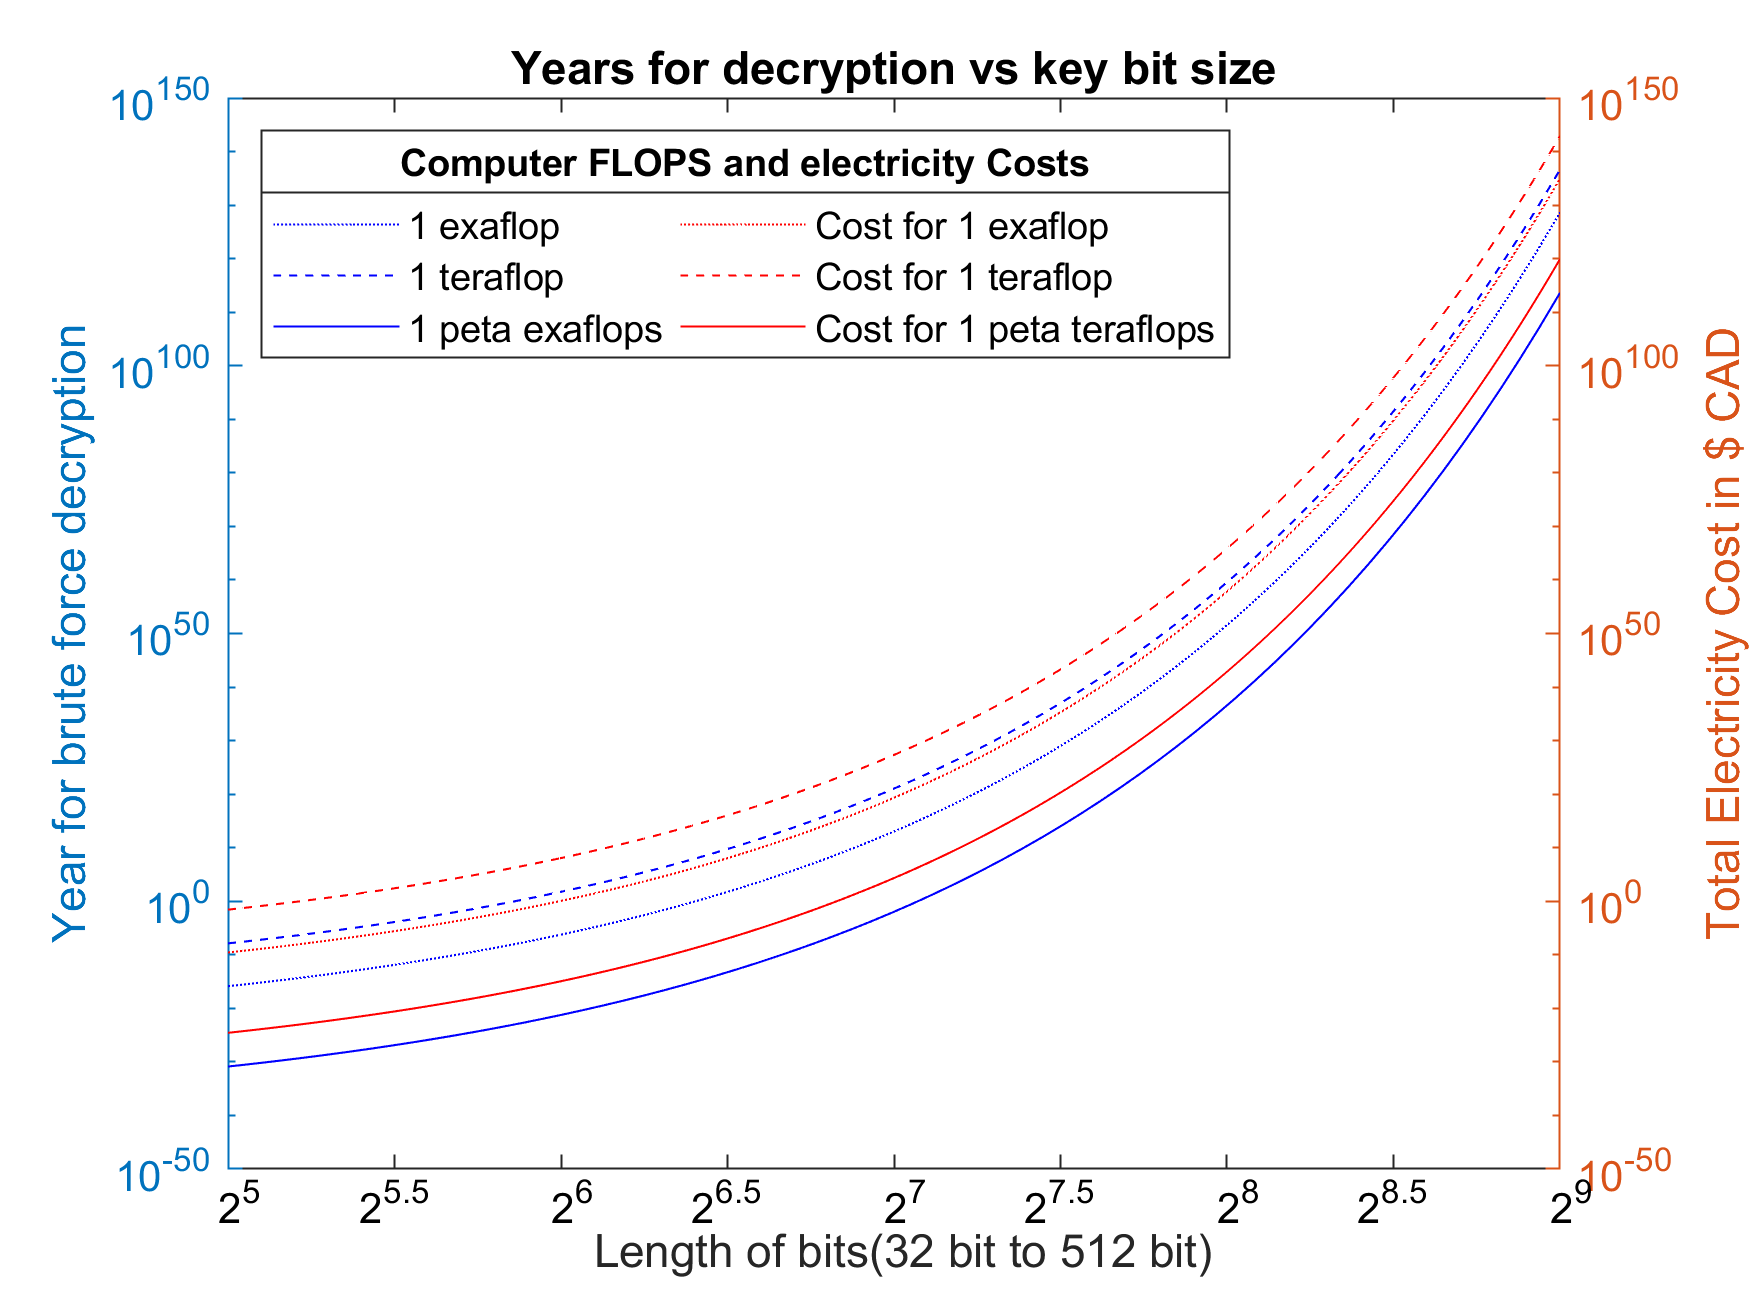
\includegraphics[width=0.7\linewidth]{Diagrams/epicPic.png}
  	\caption{Difficulty of brute forcing a 256-bit key for different computers}
  	\label{security:fig2}
  	\end{figure}


Scalability is the biggest issue facing blockchain technology, because storage is expensive, and public blockchains are trustless, every transaction is verified \cite{ethScale:Online}. 

\subsubsection{Enforcability of Smart Contracts}



If contractual fulfillment are delegated to code, it becomes paramount to
ensure that such code contains no errors.  Oftentimes smart contracts run on top of a blockchain, so the code of the smart contract would be neither incorruptible nor secure. When self-enforcement guarantees performance and subsequent human intervention is disallowed, modification of a  smart contract is impossible, logically, its
code must be perfect. 

Lastly, it must be acknowledged that self-enforcement may be limited to transactions
where off-chain events are computationally verifiable. Just like not all contractual
obligations can be represented in code, not all off-chain events can be captured as
computer-readable data or measured with objective criteria. 

\subsubsection{Performance of Smart Contracts}
Statistically, every computer program coding error ("bugs"). It is practically impossible to ensure perfect performance of a smart contract. Immutable, self-executing smart contracts may protect  
the transaction from unexpected human interactions but introduce the risk of
performance being affected by coding errors. Given that the smart contract may execute incorrectly due to a coding error, the practical difficulty of writing bug-free code, alleviating and reducing risk from vulnerabilities is essential.


% Rewrite heavily 
Technical writings suggest
that such direct coding of smart contracts would force lawyers to be more precise and
structured in describing the rights and obligations of the parties \cite{stepWolf}. Since most lawyers are unlikely to become programmers and vice-verse, converting existing legal documents into smart contracts is undesirable. In order to create smart contracts, obligations must be reported in a  detailed manner and provide objective criteria for execution.


\subsubsection{Transparency and Speed of Blockchain Transactions}

	
Disadvantages of blockchain data storage include difficult retrieving relevant information (without an abstraction layer, the entire blockchain or a single transaction is returned), users will experience latency before transactions are validated, 	\footnote{For bitcoin, it takes 10 minutes before blocks of transactions are validated (mining process)} and writing to the blockchain is relatively expensive compared to traditional systems. Smart contracts are useful because they cannot be changed by the parties involved in the transactions, yet, in some cases such as criminal activity, the ability to reverse transactions or freeze accounts is extremely desirable. For example EOS, a centralized blockchain platform, was criticized for freezing accounts without due process and community backing. \cite{EOS:Online}. %In addition, centralized systems require users to trust vendors and oftentimes personal data usage lacks transparency.
%In this sense, smart
%contracts could in fact reduce ambiguity because must be capable of a single
%interpretation. Given that most lawyers are unlikely to become programmers (just as
%most programmers are unlikely to become skilled drafters), it is suggested that even if
%smart contracts cannot be coded directly, contracts could be drafted with encoding in
%mind. To this end, the contracting parties (and their lawyers) could reorient the
%manner in which they express their agreement to facilitate its subsequent translation
%into code,
%73 e.g. describe their obligations in a formalized, structured manner and
%provide objective, measurable criteria that must be met for such obligation to be
%considered performed. 
%38 An interesting result follows: as neither party can interfere with the operation of the smart contract, breach is technically impossible – at least if breach is associated with an event that is somehow
%related to or within the control of the parties. The smart contract may, however,
%execute incorrectly due to a coding error. In such instance, it seems more
%appropriate to speak of a malfunction than of breach. Given the practical difficulty of
%preventing such malfunctions, it may be necessary to allocate the risk of their
%occurrence by prior agreement. 
%
%